%%%
% Interactive Semi-automatic Layout
%%%

\section{Interaktives halbautomatisches Layout}
\label{sec:interactive-semi-automatic-layout}

Wie bereits in diesem Kapitel präsentiert wurde, unterstützen die meisten Editoren zur Erstellung von Diagrammen Hilfefunktionen für das manuelle Layout (Abschnitt \ref{sec:manual-layout}) und eventuell auch automatische Layout-Algorithmen (Abschnitt \ref{sec:automatic-layout}). Das manuelle Layout ist sehr intuitiv, zeichnet sich durch die direkte Interaktion des Nutzers mit dem Diagramm aus, vermisst aber eine automatisierte Layout-Berechnung und Berücksichtigung der ästhetischen Prinzipien. Dieses Problem wird durch das automatische Layout bekämpft, das aber in dem Bereich der Interaktivität versagt \cite{GladischSchumann14Semi-Automatic}. Die Vorteile der Ansätze aus beiden genannten Kategorien lassen sich kombinieren und bilden eine neue Kategorie der Ansätze für die halbautomatische Layout-Unterstützung.

Diese Ansätze sind für Nutzer-bedingte Änderungen ausgelegt und ermöglichen eine inkrementelle Erstellung der Diagramme mit Bezug auf das Layout. Somit sind sie insbesondere für interaktive Umgebungen geeignet \cite{Arvo02Techniques, GladischSchumann14Semi-Automatic, Wybrow08Using}.


% dynamische Algorithmen, Sequenzen von Modifizierungen
% Nutzer kann einige Aspekte des Layouts beeinflussen, z.B. durch direkte Positionierung der Knoten bzw. Kanten oder durch eine Form von Feedback [Arvo02]
% inkrementelles Layout

\subsection{Struktur-basierte benutzergesteuerte Ansätze}
\label{structure-based-user-controlled-approaches}

Die erste Kategorie der Ansätze für das interaktive halbautomatische Layout bilden die Struktur-basierten benutzergesteuerten Ansätze, die dem Nutzer ermöglichen, das Layout des Diagramms durch Erstellung und Verwaltung von Strukturregeln\footnote{Ein Beispiel für eine solche Strukturregel ist die im Abschnitt \ref{subsubsec:alignment-and-distribution} beschriebene gleichmäßige Verteilung der ausgewählten Objekte in Relation zueinander.} zu beeinflussen. Diese Strukturregeln erinnern an die Hilfefunktionen für das manuelle Layout (siehe Abschnitt \ref{subsec:help-functions-for-manual-layout}), sind aber dahingegen persistent \cite{Wybrow08Using}. Sie werden bei der Berechnung des Layouts durch einen dynamischen Layout-Algorithmus berücksichtigt und eingehalten.

Die Struktur-basierten benutzergesteuerten Ansätze lassen sich in zwei Gruppen unterteilen: in Constraint-basierte und Pattern-basierte Ansätze. Beide Gruppen werden im Folgenden vorgestellt.

\subsubsection{Constraint-basierte Ansätze}
\label{subsubsec:constraint-based-approaches}

Die Strukturregeln können mit Hilfe von Constraints umgesetzt werden. Ein valides Layout wird dadurch berechnet, in dem alle Constraints im Diagramm mit einem Constraintlöser ausgewertet werden.



% deklarativ
% welche Regeln sollen gelten anstatt wie
% Constraintlöser, verschiedene Typen (beschrieben in [Mai])

% Cassowary for layout of UI in Cocoa/iOS

% Dunnart: Screenshot, http://dunnart.org
% Nutzer kann Constraints erstellen und auf Teile des Diagramms anwenden

% Probleme mit der Performance, da der Algorithmus nach jeder kleinen Änderung laufen muss

\subsubsection{Pattern-basierter Ansatz}

Der in \cite{Maier12A-Pattern-based} und \cite{MaierMinas10Combination} präsentierte Pattern-basierte Ansatz für das Layout von Diagrammen drückt die Strukturregeln in Form von Layout-Patterns aus. Der Ansatz kann für beliebige visuellen Sprachen eingesetzt werden, die mit Meta-Modellen beschrieben werden können. Dabei besteht das sprachenspezifische Meta-Modell aus zwei Teilen, nämlich der Meta-Modelle für die abstrakte und konkrete Syntax. Das zuletzt genannte Meta-Modell beschreibt die visuellen Eigenschaften der Sprache und wird daher durch die Berechnung des Layouts beeinflusst.

Die Beschreibung der Layout-Patterns erfolgt allerdings nicht mit Hilfe der sprachenspezifischen Meta-Modellen, sondern mit sprachenunabhängigen Pattern-spezifischen Meta-Model\-len\footnote{In \cite{Maier12A-Pattern-based} werden u.a. Pattern-spezifische Meta-Modelle für Mengen von Elementen, geordnete Liste von Elementen oder Graphen vorgestellt.}. Bei der Instanziierung eines Layout-Patterns wird das sprachenspezifische Modell auf ein Pattern-spezifisches Modell abgebildet\footnote{Dieses Sachverhalt wird mit Hilfe eines Beispiels in \cite[S.59ff]{Maier12A-Pattern-based} anschaulich gemacht.}. Dadurch wird eine mögliche Wiederverwendung der Layout-Patterns für diverse visuellen Sprachen gewährleistet. Weiterhin zeichnet sich der Pattern-basierte Ansatz dadurch aus, dass die Layout-Patterns verschiedene Ansätze zum Layout von Diagrammen u.a. Algorithmen zum Graphenzeichnen (siehe Abschnitt \ref{subsubsec:graph-drawing-tools}) und Constraints-basierte Algorithmen (siehe Abschnitt \ref{subsubsec:constraint-based-approaches}) kombinieren und sich zu Nutze machen.


% Auflistung der Layout-Patterns: tree layout, layered layout, equal distance, alignment…

%Kontroll-Algorithmus läuft im Hintergrund nach jeder Änderung des Diagramms bzw. der Instanziierung eines Layout-Patterns

% benutzergesteuert, nicht eingeschränkt in Interaktion

%Wie bereits erwähnt, ist dieser Ansatz für interaktive


% Videos: http://www.sonjamaier.de/dyndraw/screencasts/graphEditor.mov & http://www.sonjamaier.de/dyndraw/screencasts/ecoreEditor.mov

Dieser Ansatz wurde in Form eines Layout-Frameworks\footnote{\url{http://www.unibw.de/inf2/Personen/Wissen_Mitarbeiter/sonja/research/layoutframework}} implementiert, das bisher noch nicht veröffentlicht wurde. Dennoch wurde es in visuellen Editoren eingesetzt, die mit Hilfe von DiaMeta\footnote{Ein Framework zur Generierung von Editoren für visuelle Sprachen basierend auf Spezifikationen mittels Meta-Modelle. \url{http://www.unibw.de/inf2/DiaGen/}} bzw. Graphical Editing Framework\footnote{\url{http://www.eclipse.org/gef/}} erzeugt wurden \cite{Maier12A-Pattern-based}.

\subsection{Anwendungsspezifische Ansätze}

Die Struktur-basierten benutzergesteuerten Ansätze für das halbautomatische Layout, die im Abschnitt \ref{structure-based-user-controlled-approaches} beschrieben wurden, sind sehr universell und können in Editoren für verschiedene visuellen Sprachen eingesetzt werden. Aus diesem Grund können die syntaktischen und semantischen Eigenschaften der Sprachen nicht gründlich in den Algorithmen berücksichtigt werden. Dahingegen gibt es anwendungsspezifische Ansätze, deren Algorithmen für konkrete visuelle Sprachen entworfen sind. Diese werden im Folgenden vorgestellt.

\subsubsection{Smart Layout in MindNode}

MindNode\footnote{\url{https://mindnode.com}} ist ein benutzerfreundliche Desktop-Anwendung zur Erstellung von Mind-Maps für Mac OS X. Die Mind-Maps haben eine baumbasierte Struktur mit einem oder mehreren zentralen Knoten. Weiterhin gilt, dass jeder Knoten mehrere Unterknoten besitzen kann und alle Knoten außer den zentralen Knoten haben genau einen Oberknoten. Die hierarchischen Relationen werden mit farbigen Zweigen dargestellt. Zusätzlich bietet MindNode die Möglichkeit der Querverbindungen zwischen Knoten aus unterschiedlichen Teilen der Mind-Map, die mit gestrichelten Pfeilen gekennzeichnet werden \cite{14MindNode}. In Abbildung \ref{fig:mindnode-example} ist ein Beispiel einer Mind-Map zu sehen.

\begin{figure}[hbt]
    \centering
    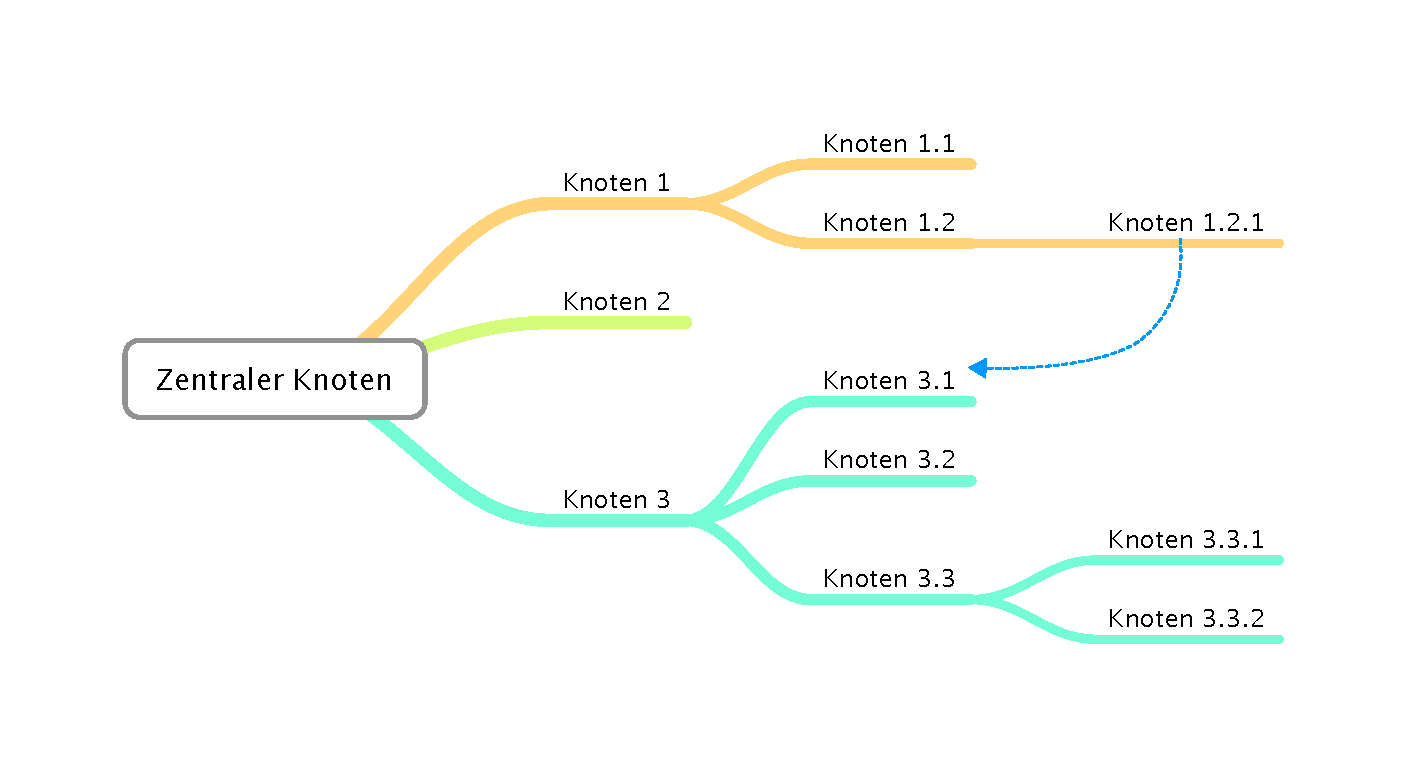
\includegraphics[
        width=\textwidth,
        trim={0 1.5cm 0 1.5cm},
        clip
    ]{resources/mindnode-example}
    \caption{Beispiel einer Mind-Map in MindNode}
    \label{fig:mindnode-example}
\end{figure}

MindNode stellt eine interaktive Funktion für eine halbautomatische Layout-Unterstützung namens \enquote{Smart Layout} bereit \cite{14MindNode}. Wenn diese Funktion ausgeschaltet ist, können einzelne Knoten der Mind-Map frei positioniert werden. Dahingegen, wenn die Funktion eingeschaltet ist, nimmt die Mind-Map eine vorgerechnete Baumstruktur an und die Verschiebungsoperation eines Knotens drückt in diesem Fall die Absicht einer Layout-Modifikation aus.

In Abbildung \ref{fig:mindnode-smart-layout} wird die Funktionsweise der Funktion \enquote{Smart Layout} anhand von Screenshots gezeigt. Zunächst wird in \ref{fig:mindnode-smart-layout-a} ein Knoten angeklickt, dessen Position angepasst werden soll. Mit \enquote{Drag an Drop} wird in \ref{fig:mindnode-smart-layout-b} der Knoten auf die gewünschte Position verschoben. Die Verbindung zu dem Oberknoten wird dabei mit einem heller gemachten Zweig veranschaulicht. Nach dem Loslassen der Maustaste in \ref{fig:mindnode-smart-layout-c} wird die gewünschte Position der verschobenen Knotens ausgewertet, ein neues Layout der Mind-Map anhand des Hinweises durch die Verschiebungsoperation berechnet und anschließend auf die Mind-Map angewendet, indem alle beeinflussten Knoten von ihren aktuellen Position zu ihren neuen Position animiert werden. Somit kann der Nutzer das Layout beeinflussen, wird aber in den Möglichkeiten eingeschränkt. Dies führt in der Regel zu einem optimalen Layout und ist vor allem durch die Struktur der visuellen Sprache für Mind-Maps möglich.

% Unterknoten des zentralen Knotens können auf die linke bzw. rechte Seite verschoben werden
% initiales Layout

% TODO: Mauszeiger hinzufügen
\begin{figure}[hbt]
    \newcommand{\subfigurewidth}{\textwidth}
    \newcommand{\graphicswidth}{0.8\linewidth}
    \begin{subfigure}{\subfigurewidth}
        \centering
        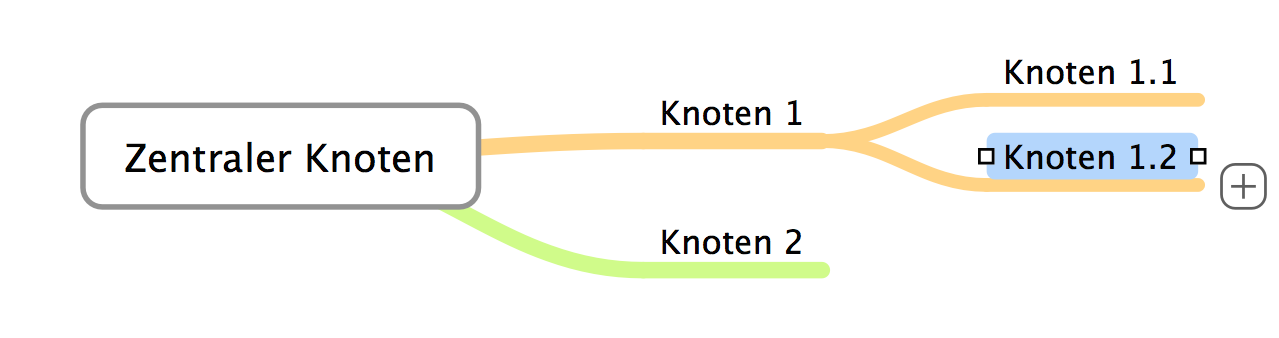
\includegraphics[width=\graphicswidth]{resources/mindnode-smart-layout-a}
        \caption{Auswahl des Knotens}
        \label{fig:mindnode-smart-layout-a}
    \end{subfigure}
    \begin{subfigure}{\subfigurewidth}
        \centering
        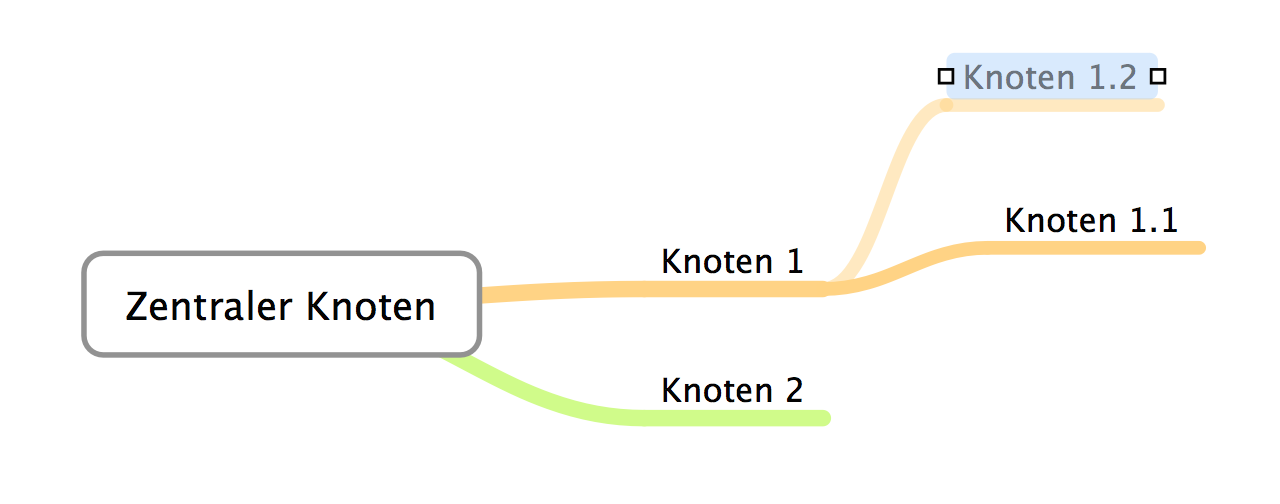
\includegraphics[width=\graphicswidth]{resources/mindnode-smart-layout-b}
        \caption{Verschiebung des ausgewählten Knoten}
        \label{fig:mindnode-smart-layout-b}
    \end{subfigure}
    \begin{subfigure}{\subfigurewidth}
        \centering
        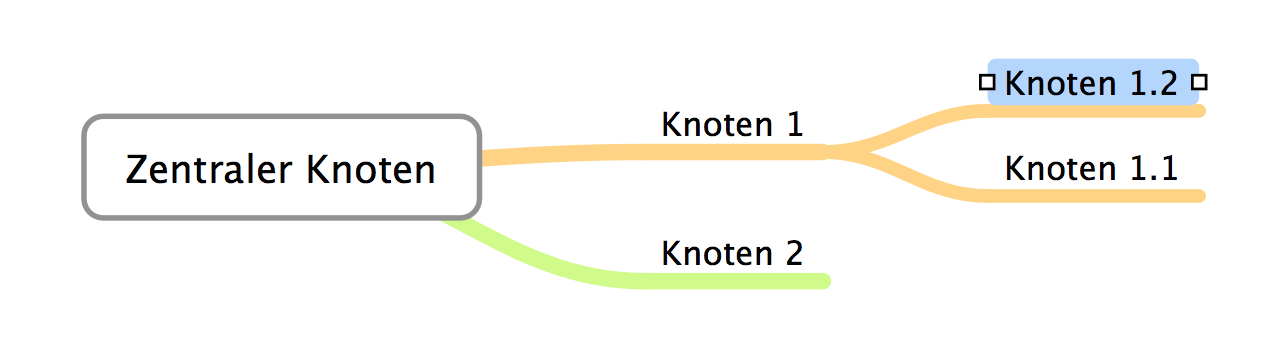
\includegraphics[width=\graphicswidth]{resources/mindnode-smart-layout-c}
        \caption{Neue Positionen der Knoten}
        \label{fig:mindnode-smart-layout-c}
    \end{subfigure}
    \caption{Eine Verschiebungsoperation mit der eingeschalteten Funktion \enquote{Smart Layout} in MindNode}
    \label{fig:mindnode-smart-layout}
\end{figure}

\subsection{Eigenschaften und Vergleich}

% Wahrnehmungsorganisation hat eine größere Priorität als reine Berücksichtigung der syntaktischen Ästhetik [Shieber]
% Beides Kombinieren [Shieber]

% Nur visualisieren vs. auch Editieren [Gladisch]
% Nutzer entwickeln ein mentales Modell des Diagramms, das soll bei den inkrementellen Updates berücksichtigt werden [Gladisch]

% Der Nutzer kann das Diagramm unmittelbar bearbeiten
% das mentale Modell bleibt beibehalten [preserving the mental map (in dynamic context) instead of aesthetics (in static context)]
% ästhetische Regeln werden nicht eingehalten







